\chapter{Khám Phá Dữ Liệu (EDA) \& Tiền Xử Lý}
\label{chap:eda}

\section{Tổng Quan Tập Dữ Liệu \& Quy Trình Tiền Xử Lý}
Tập dữ liệu do Ban tổ chức cung cấp bao gồm:
\begin{itemize}
  \item \textbf{Tập huấn luyện (Train set):} 2.494 bài báo khoa học với các trường thông tin: \texttt{id}, \texttt{title}, \texttt{venue}, \texttt{year}, \texttt{authors}, \texttt{doi}, và nhãn đánh giá \texttt{Label} $\in \{1, 2, 3, 4, 5\}$.
  \item \textbf{Tập kiểm thử (Test set):} 596 bài báo ứng viên với cùng các trường thông tin trên, ngoại trừ trường \texttt{Label} bị ẩn.
\end{itemize}

\subsection{Làm Sạch Văn Bản \& Xử Lý Giá Trị Khuyết}
Qua quá trình kiểm tra toàn vẹn dữ liệu (\textit{Data Sanity Check}), nhóm đã phát hiện và xử lý các vấn đề kỹ thuật sau:
\begin{enumerate}
  \item \textbf{Giải mã thực thể HTML trong tiêu đề bài báo:} Nhiều tiêu đề bài báo xuất phát từ nguồn trích xuất tự động chứa các thực thể HTML mã hóa như \texttt{\&apos;} (dấu nháy đơn), \texttt{\&quot;} (dấu ngoặc kép), \texttt{\&amp;} (dấu và), \texttt{\&lt;}, \texttt{\&gt;}. Nếu không giải mã, các mô hình ngôn ngữ và TF-IDF sẽ phân tách sai cấu trúc từ vựng. Nhóm đã sử dụng thư viện \texttt{html.unescape()} và chuẩn hóa khoảng trắng dư thừa cho $100\%$ tiêu đề.
  \item \textbf{Xử lý trường tác giả (\texttt{authors}):} Khoảng $1.8\%$ bài báo bị khuyết trường tác giả (thường là bài kỷ yếu hoặc báo cáo tổng kết). Với các bài này, chuỗi tác giả được điền giá trị rỗng \texttt{""} và số lượng tác giả được gán bằng $0$.
  \item \textbf{Xử lý trường định danh DOI (\texttt{doi}):} Có khoảng $18.5\%$ bài báo không có mã DOI. Nhóm tạo một biến cờ nhị phân $\texttt{has\_doi} \in \{0, 1\}$ để nắm bắt thông tin xuất bản chính thống.
  \item \textbf{Chuẩn hóa năm xuất bản (\texttt{year}):} Các giá trị năm khuyết hoặc không hợp lệ được gán bằng trung vị lịch sử (năm 2020), sau đó chuẩn hóa tuyến tính về đoạn $[-0.5, 0.5]$: $\text{year\_norm} = (\text{year} - 2000) / 30$.
\end{enumerate}

\section{Phân Tích Trực Quan Khám Phá Dữ Liệu (EDA)}

\subsection{Phân Phối Nhãn Đánh Giá (\texttt{Label})}
Hình \ref{fig:label_dist} thể hiện phân phối tần suất của 5 mức đánh giá trong tập huấn luyện 2.494 bài báo.

\begin{figure}[!ht]
  \centering
  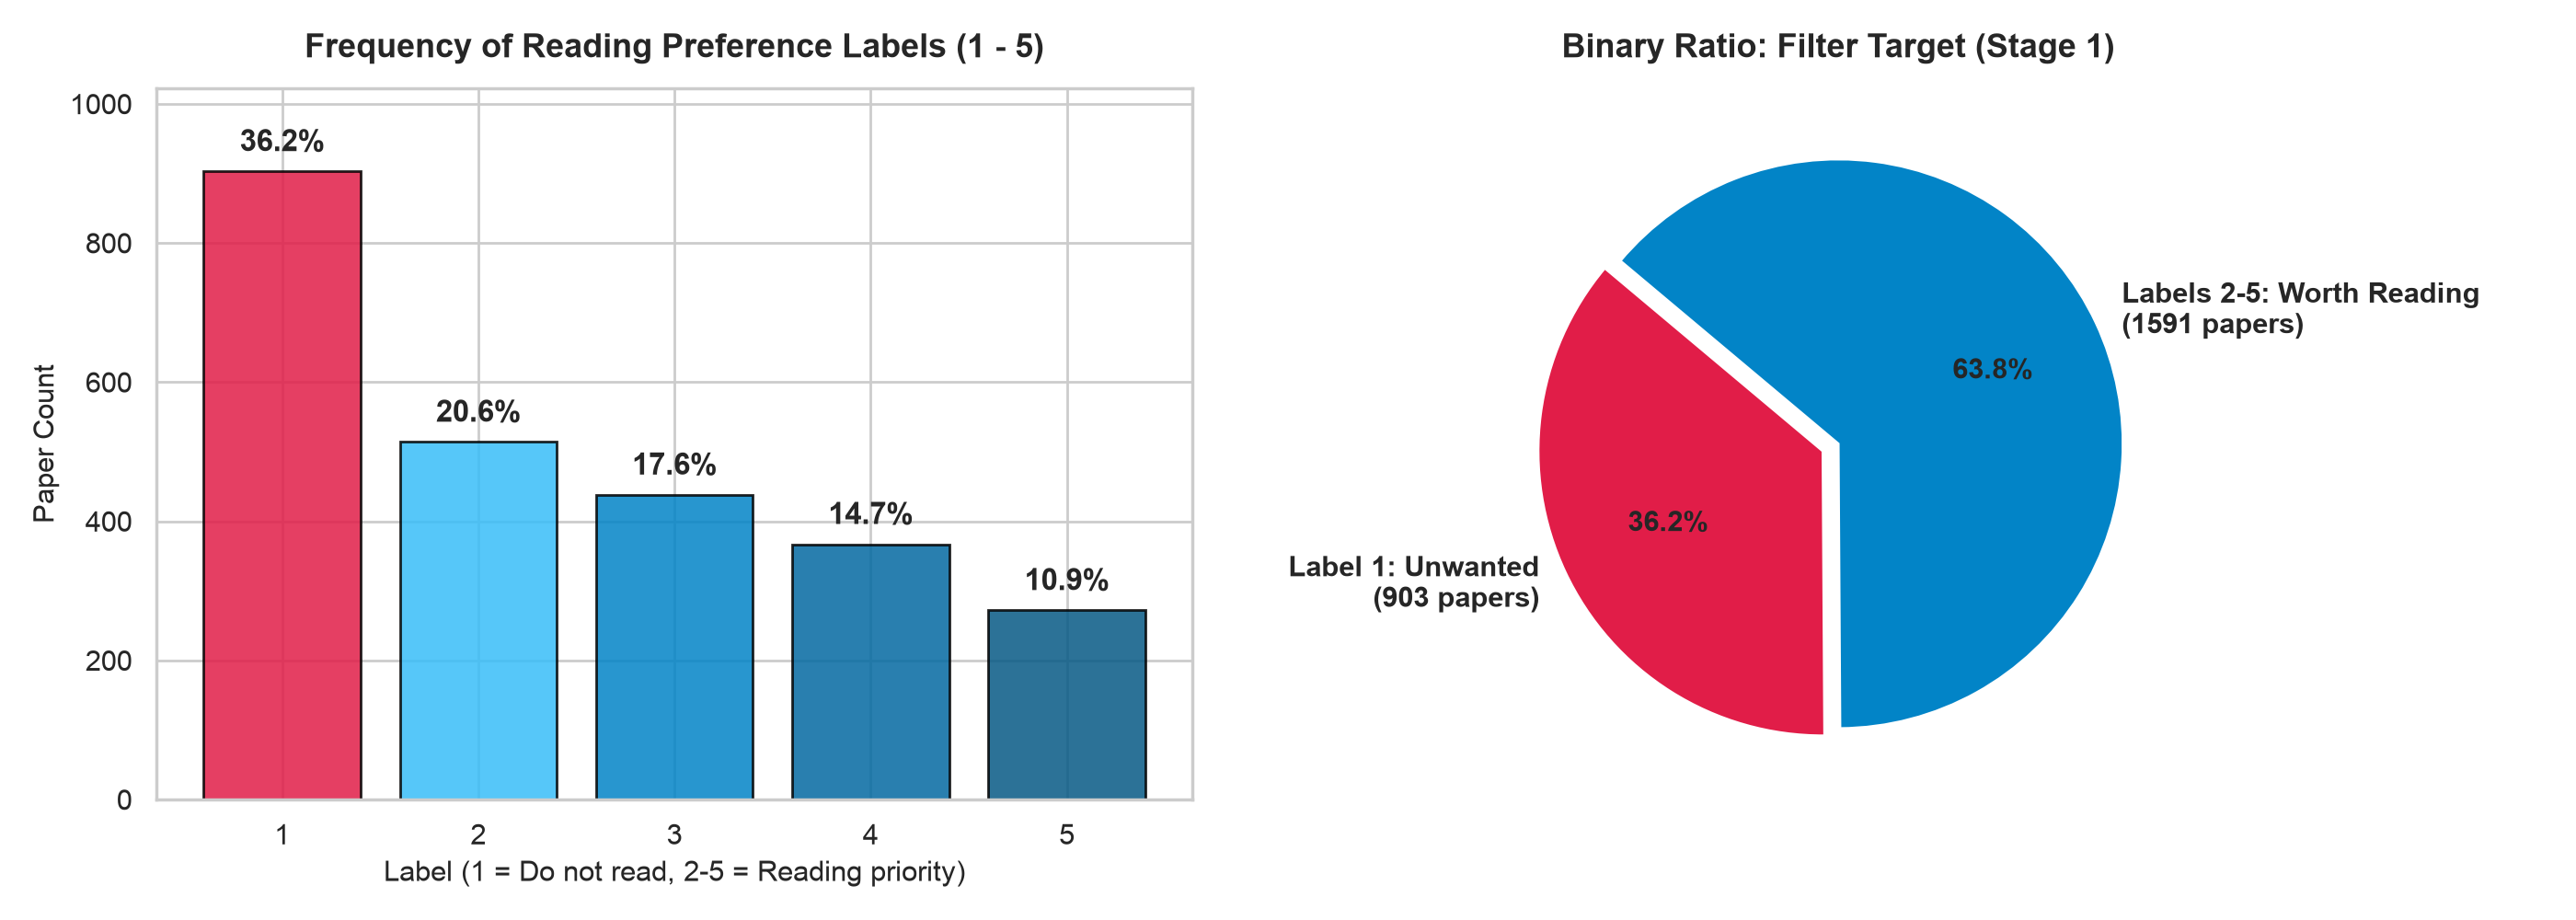
\includegraphics[width=0.75\linewidth]{figures/01_label_distribution.png}
  \caption{Phân phối tần suất và tỷ lệ phần trăm các mức đánh giá (Nhãn 1 đến 5)}
  \label{fig:label_dist}
\end{figure}

\begin{itemize}
  \item \textbf{Nhãn 1 (Không muốn đọc):} Chiếm số lượng áp đảo với 903 bài báo (**$36.2\%$**). Điều này phản ánh thực tế rằng trong một danh mục bài báo tổng hợp, phần lớn các bài không thuộc mối quan tâm của nhà nghiên cứu.
  \item \textbf{Nhãn 2--5 (Bài đáng đọc):} Chiếm $63.8\%$ tổng thể (1.591 bài), trong đó số lượng giảm dần theo mức độ ưu tiên: Nhãn 2 (514 bài, $20.6\%$), Nhãn 3 (438 bài, $17.6\%$), Nhãn 4 (367 bài, $14.7\%$), và Nhãn 5 (272 bài, $10.9\%$).
  \item $\implies$ \textbf{Ý nghĩa với mô hình:} Dữ liệu có sự mất cân bằng giữa bài cần lọc (Nhãn 1: 36.2\%) và bài cần giữ (Nhãn 2--5: 63.8\%). Mô hình phân loại ở Stage 1 cần đặc biệt chú ý kiểm soát tỷ lệ lỗi loại I (\textit{False Positive}) để không để lọt bài nhãn 1.
\end{itemize}

\subsection{Mối Quan Hệ Giữa Năm Xuất Bản \& Điểm Đánh Giá}
Hình \ref{fig:year_dist} phân tích sự phân bổ của điểm đánh giá theo từng năm xuất bản (từ 2016 đến 2026).

\begin{figure}[!ht]
  \centering
  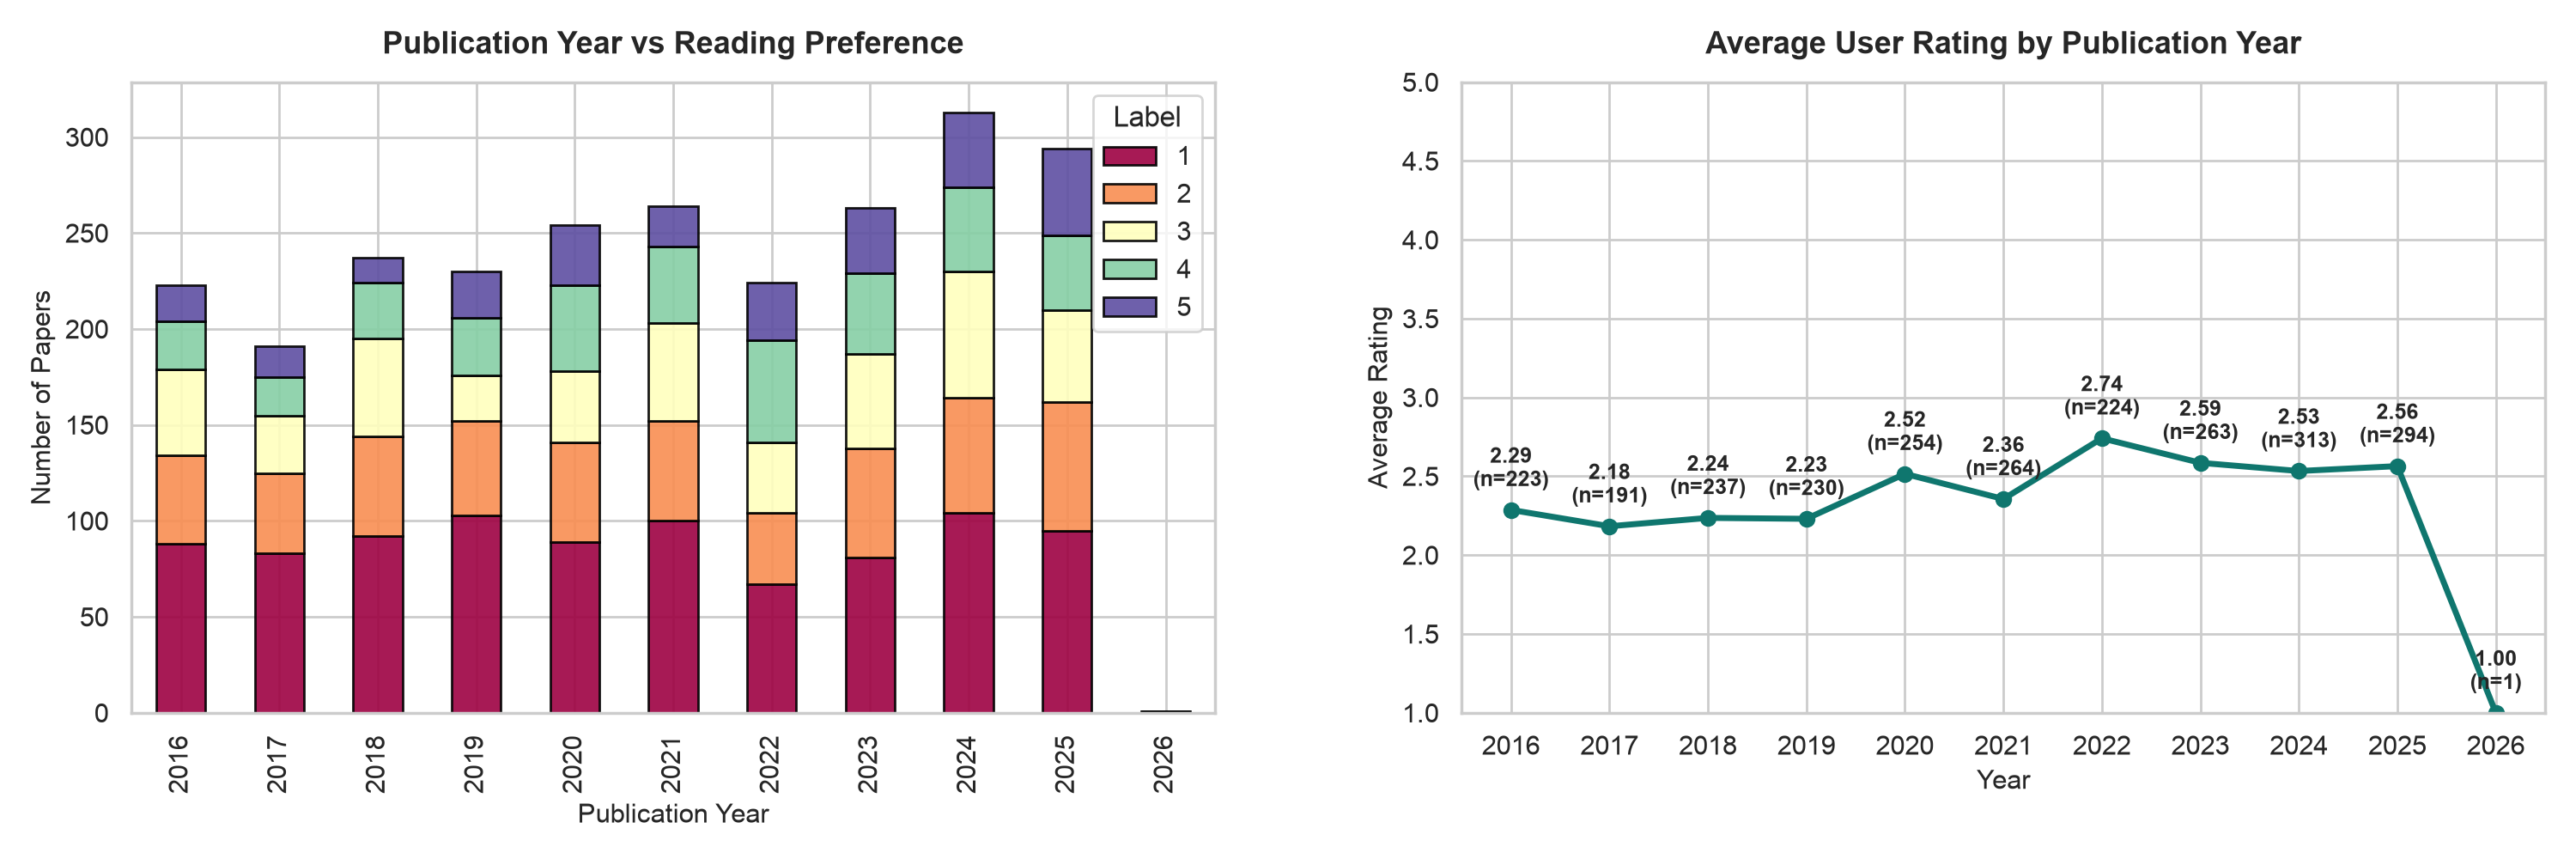
\includegraphics[width=0.76\linewidth]{figures/02_year_vs_label.png}
  \caption{Phân phối năm xuất bản phân tầng theo mức độ ưu tiên đọc}
  \label{fig:year_dist}
\end{figure}

\begin{itemize}
  \item Số lượng bài báo tập trung dày đặc nhất trong giai đoạn 2020--2025 (trung bình 250--310 bài/năm).
  \item Các bài báo xuất bản trong các năm gần đây (2022--2025) có điểm đánh giá trung bình cao hơn rõ rệt ($\approx 2.55 - 2.74$) so với các bài báo giai đoạn 2016--2019 ($\approx 2.18 - 2.23$). 
  \item $\implies$ \textbf{Nhận định:} Nhà nghiên cứu có xu hướng ưu tiên cập nhật các công trình mới nhất phản ánh các bước tiến khoa học gần đây, tạo nên tín hiệu thời gian quan trọng cho mô hình xếp hạng.
\end{itemize}

\subsection{Hiện Tượng Thiên Lệch Hội Nghị (Venue Skew Analysis)}
Hình \ref{fig:venues} thể hiện số lượng bài báo và tỷ lệ bài đáng đọc phân bổ theo từng hội nghị/tạp chí.

\begin{figure}[!ht]
  \centering
  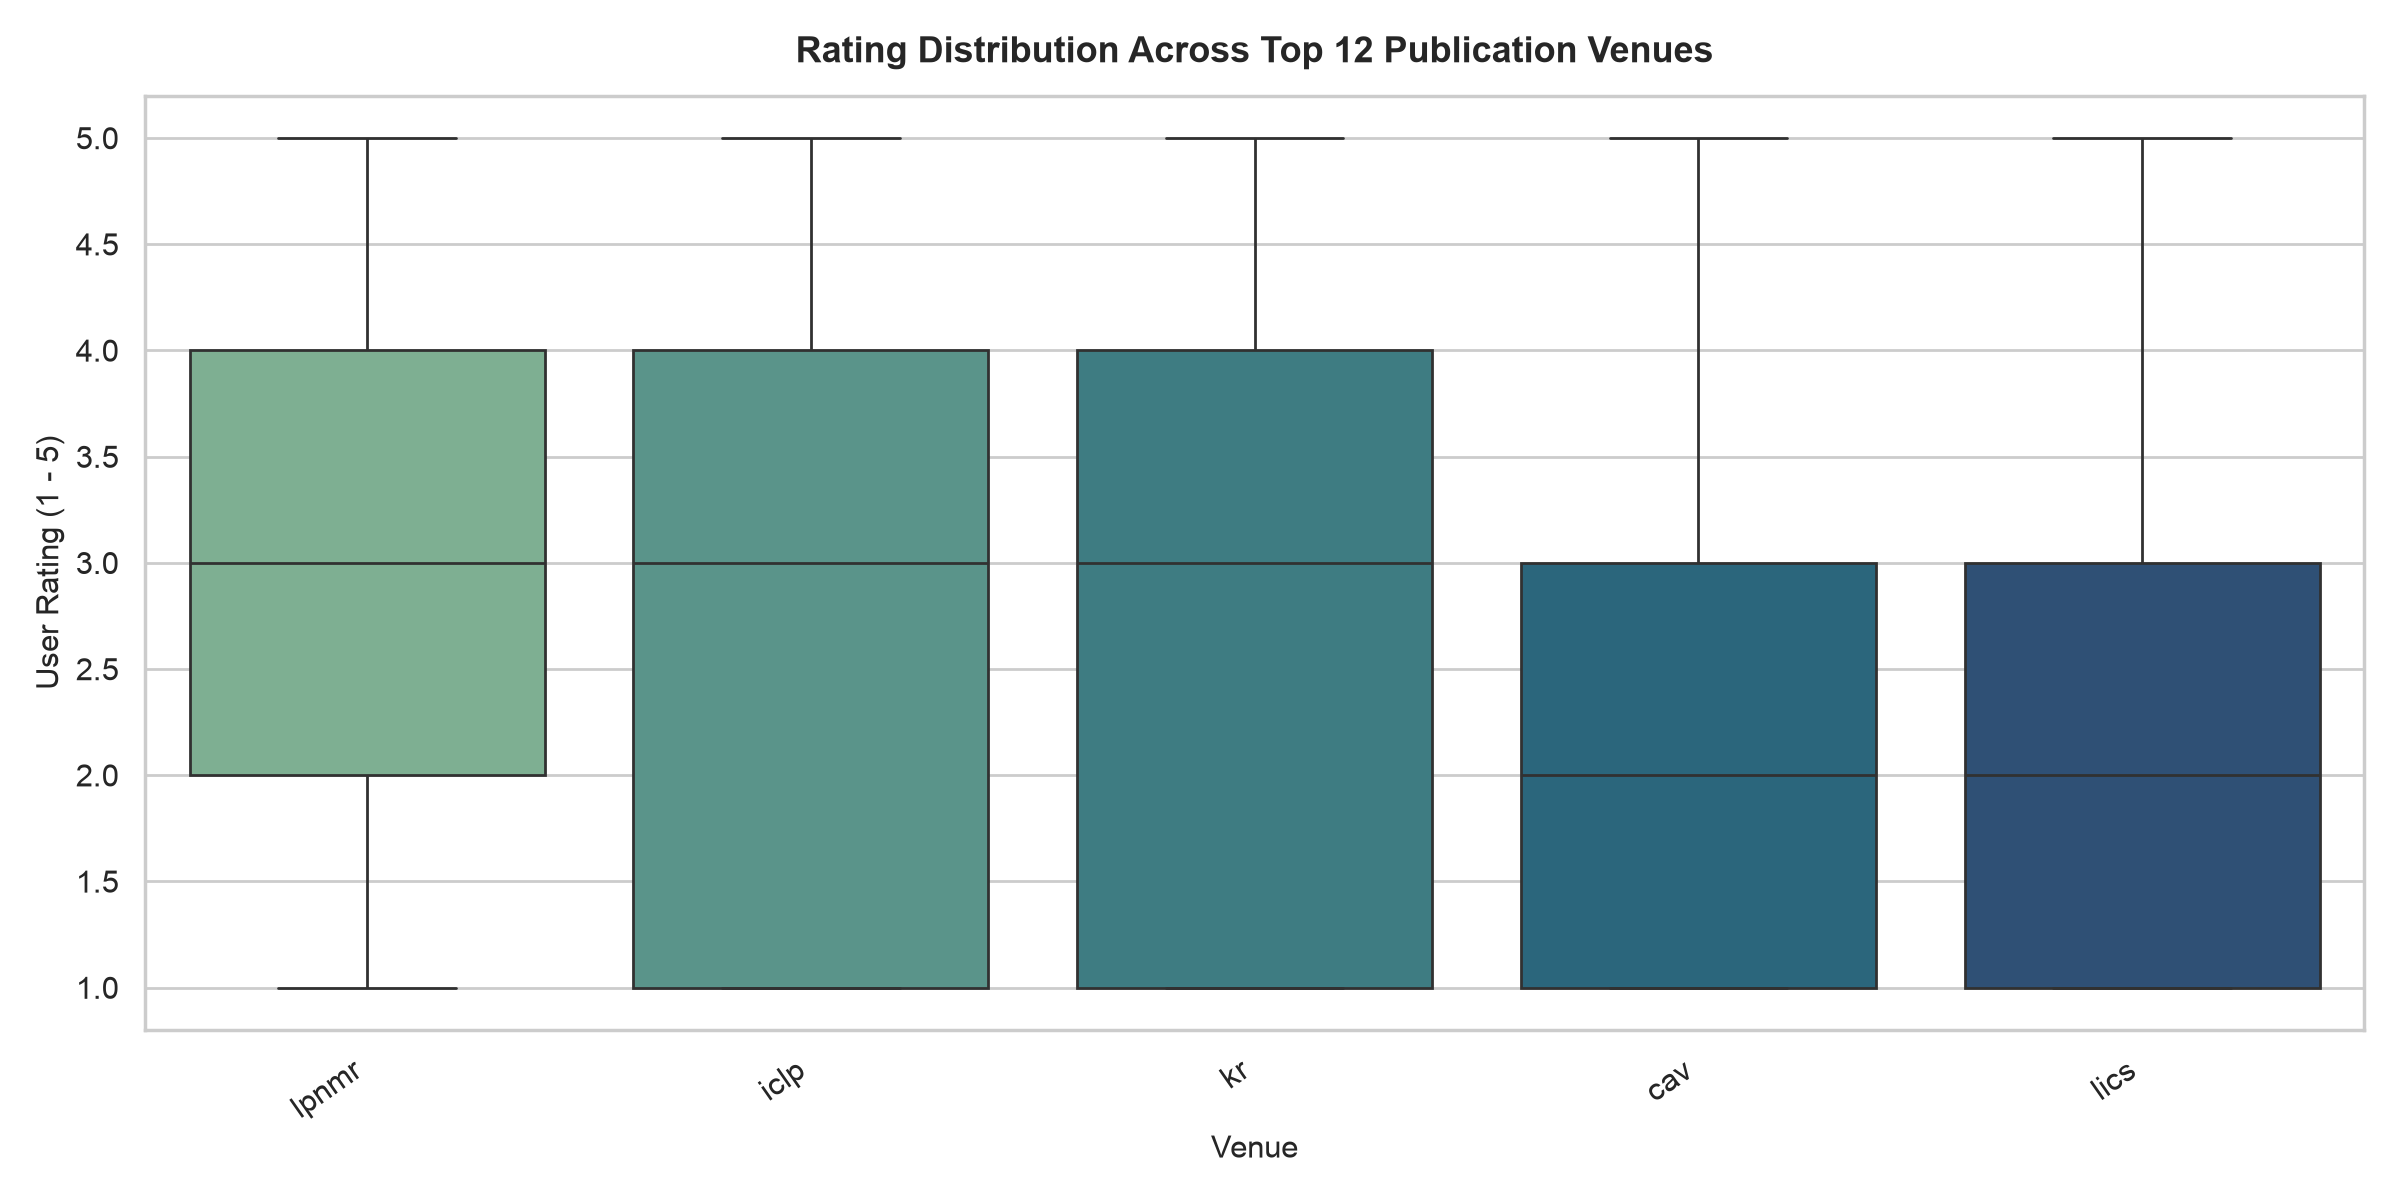
\includegraphics[width=0.75\linewidth]{figures/03_top_venues.png}
  \caption{Thống kê số lượng bài báo và điểm đánh giá trung bình theo từng hội nghị/tạp chí}
  \label{fig:venues}
\end{figure}

\begin{table}[H]
  \centering
  \small
  \begin{tabularx}{\linewidth}{>{\bfseries\raggedright\arraybackslash}p{2.5cm} >{\centering\arraybackslash}p{2.2cm} >{\centering\arraybackslash}p{2.5cm} >{\centering\arraybackslash}p{2.8cm} >{\centering\arraybackslash}p{2.5cm}}
    \toprule
    \rowcolor{PrismHeader}
    \color{PrismWhite}\textbf{Hội Nghị (\texttt{venue})} & 
    \color{PrismWhite}\textbf{Số Bài (Train)} & 
    \color{PrismWhite}\textbf{Điểm Trung Bình} & 
    \color{PrismWhite}\textbf{Tỷ Lệ Đáng Đọc ($y \ge 2$)} & 
    \color{PrismWhite}\textbf{Số Bài (Test)} \\
    \midrule
    \texttt{lpnmr} & 116 & $\mathbf{3.14}$ & $\mathbf{81.9\%}$ & 37 \\
    \rowcolor{PrismLabel}
    \texttt{iclp}  & 456 & $\mathbf{2.94}$ & $\mathbf{74.3\%}$ & 0 \\
    \texttt{kr}    & 661 & $2.73$ & $73.2\%$ & 151 \\
    \rowcolor{PrismLabel}
    \texttt{cav}   & 657 & $2.12$ & $54.3\%$ & $\mathbf{221}$ ($37.1\%$) \\
    \texttt{lics}  & 604 & $1.94$ & $52.3\%$ & $\mathbf{187}$ ($31.4\%$) \\
    \bottomrule
  \end{tabularx}
  \caption{So sánh thống kê tỷ lệ nhãn theo Venue giữa tập huấn luyện và tập kiểm thử}
  \label{tab:venue_stats}
\end{table}

\begin{prismbox}[title=\textbf{Phát Hiện Quan Trọng Về Venue Skew Trong Tập Test}]
Bảng \ref{tab:venue_stats} chỉ ra một sự phân hóa cực kỳ sâu sắc:
\begin{itemize}
  \item Các hội nghị thuần về Logic Programming và Lập trình tập ràng buộc (\texttt{lpnmr}, \texttt{iclp}) có tỷ lệ bài đáng đọc lên tới $74\% - 82\%$.
  \item Ngược lại, các hội nghị về Kiểm chứng mô hình (\texttt{cav}) và Logic lý thuyết (\texttt{lics}) chỉ có khoảng $52\% - 54\%$ bài đáng đọc.
  \item \textbf{Điểm hiểm hóc trong tập Test:} Hai hội nghị \texttt{cav} và \texttt{lics} lại chiếm tới $\mathbf{68.5\%}$ tổng số bài trong tập Test (408 trên tổng số 596 bài)! 
  \item Nếu mô hình không áp dụng đặc trưng thống kê mục tiêu (\textit{Target Encoding}) cho Venue, nó sẽ dễ dàng gán điểm ưu tiên quá đà cho các bài ở hai hội nghị này, làm lọt nhãn 1 và kéo sập chỉ số $Q$.
\end{itemize}
\end{prismbox}

\subsection{Phân Tích Độ Dài Tiêu Đề Bài Báo}
Hình \ref{fig:title_length} phân tích tương quan giữa độ dài tiêu đề (số từ và số ký tự) với từng nhãn đánh giá.

\begin{figure}[!ht]
  \centering
  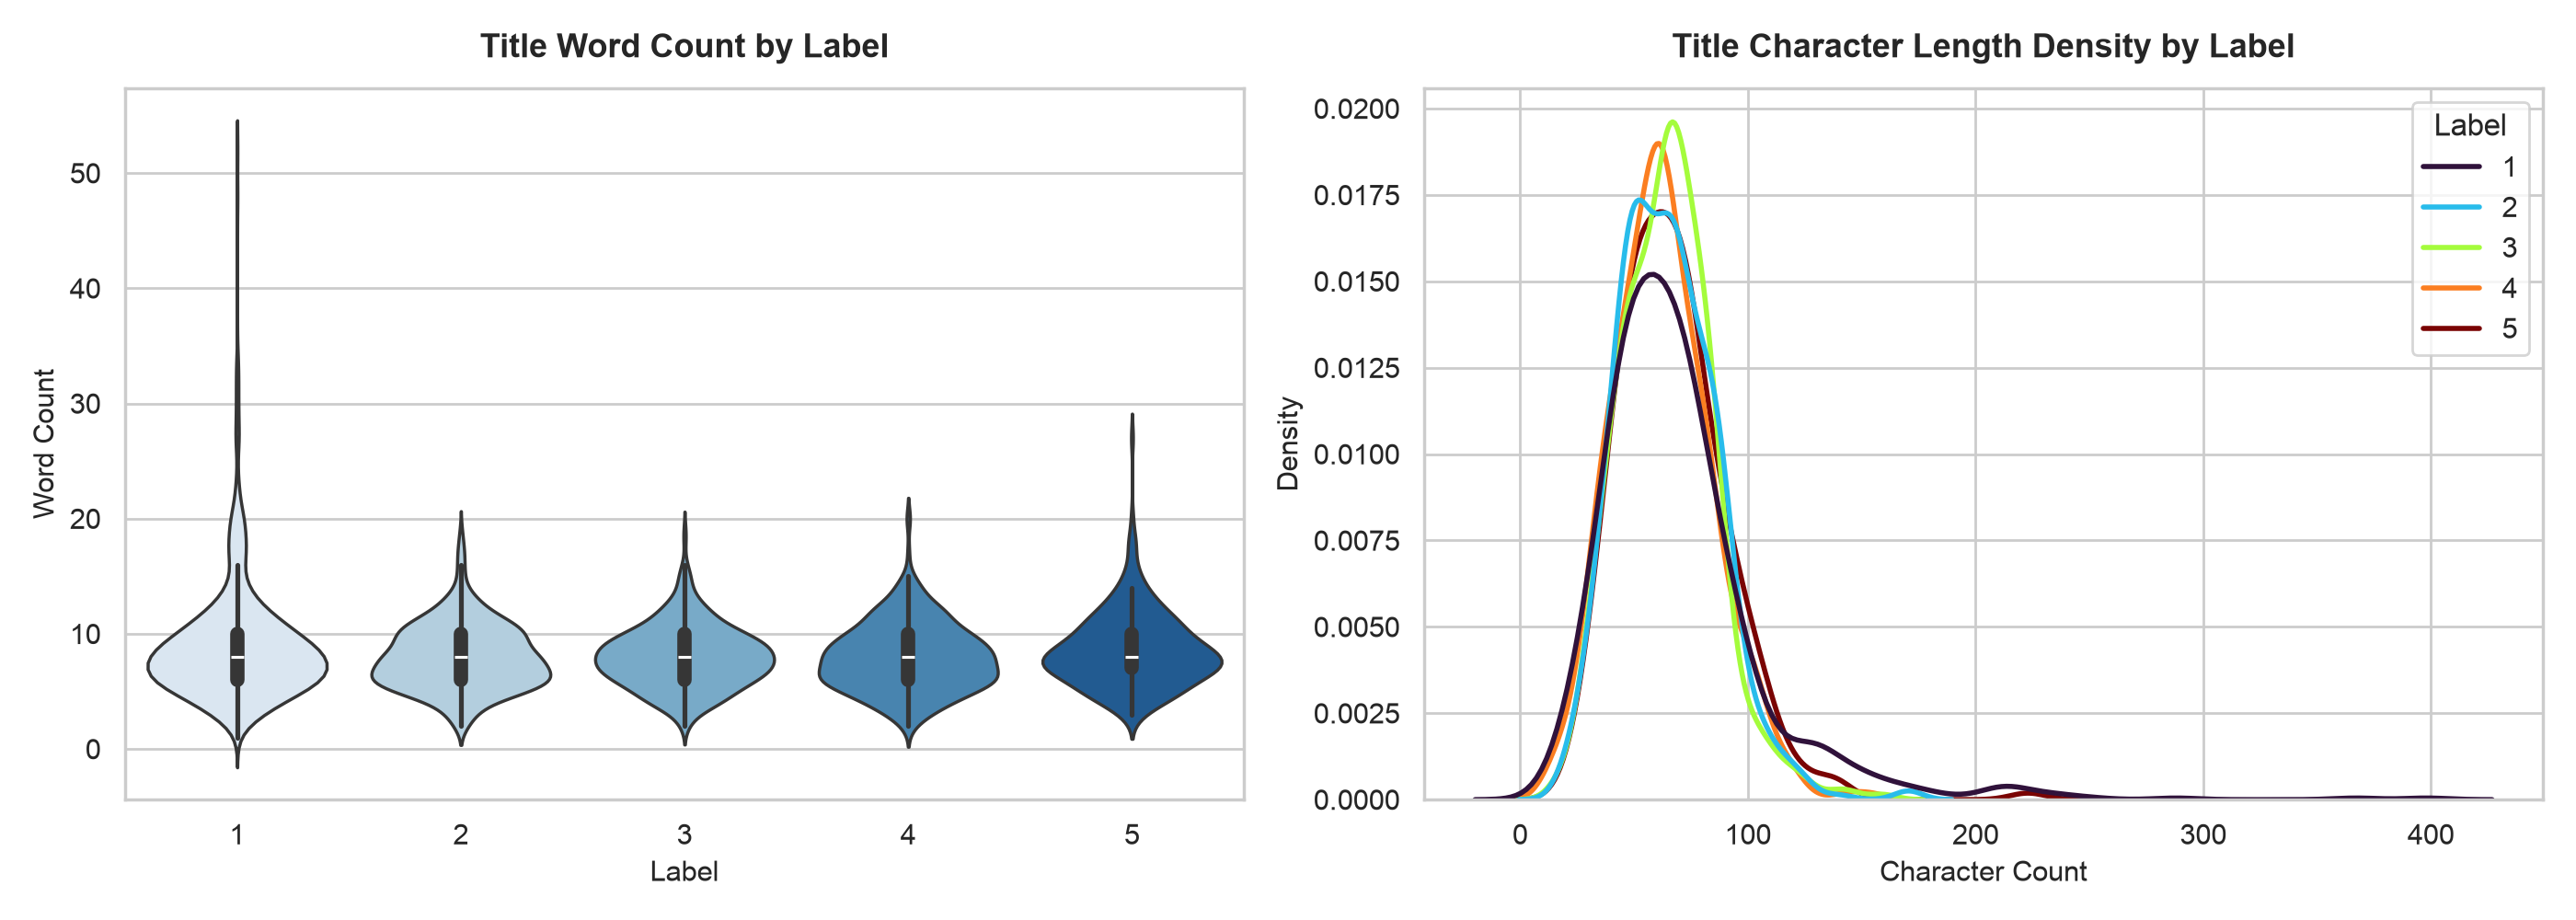
\includegraphics[width=0.76\linewidth]{figures/04_title_length_analysis.png}
  \caption{Phân phối độ dài tiêu đề (số lượng từ và số ký tự) theo từng nhãn đánh giá}
  \label{fig:title_length}
\end{figure}

\begin{itemize}
  \item Tiêu đề các bài báo khoa học có độ dài trung bình dao động từ 8 đến 14 từ (khoảng 60 đến 100 ký tự).
  \item Các bài nhãn 1 có phương sai độ dài rất lớn: một số bài có tiêu đề cực ngắn (2--4 từ, ví dụ *"Preface"* hay *"Invited Talk"*), trong khi một số khác có tiêu đề cực dài (30--50 từ, ghi rõ danh sách ban tổ chức hội nghị và địa điểm tổ chức).
  \item Tiêu đề các bài nhãn 4 và 5 có độ dài tập trung ổn định quanh mức 9--12 từ.
\end{itemize}

\subsection{Phân Tích Từ Khóa \& N-Gram Phân Biệt}
Hình \ref{fig:keywords} so sánh tỷ lệ xuất hiện của các cụm từ khóa (N-grams) phổ biến giữa nhóm bài báo có mức ưu tiên cao (Nhãn 4--5) và nhóm bài báo không muốn đọc (Nhãn 1).

\begin{figure}[!ht]
  \centering
  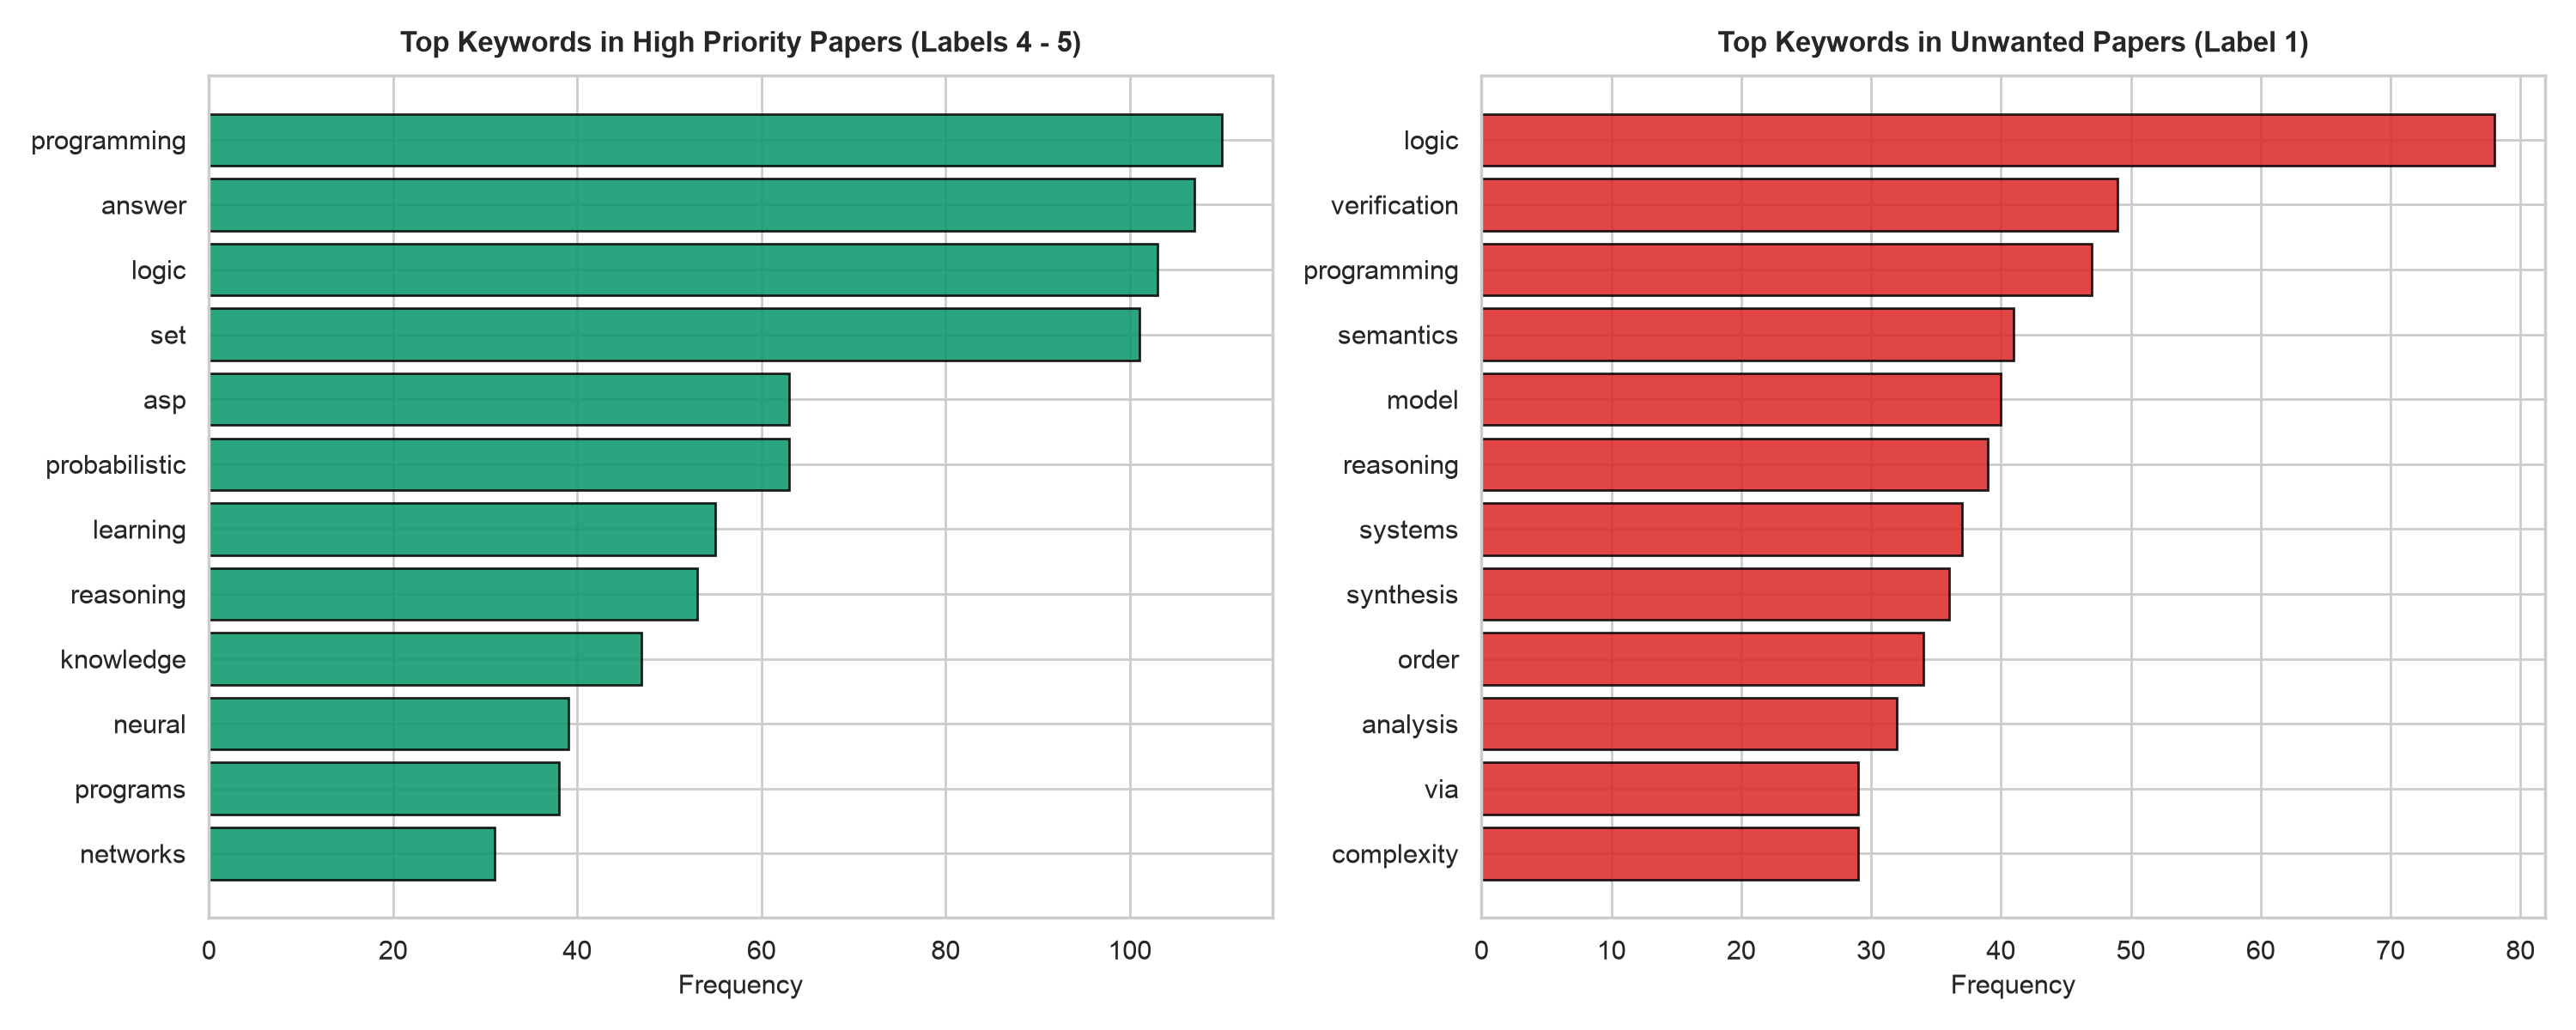
\includegraphics[width=0.76\linewidth]{figures/05_top_keywords_comparison.png}
  \caption{Tần suất xuất hiện của các từ khóa đặc trưng trong bài nhãn cao (4--5) so với nhãn 1}
  \label{fig:keywords}
\end{figure}

Phân tích định lượng tỷ số xuất hiện $\frac{\text{Tỷ lệ ở Nhãn 4-5}}{\text{Tỷ lệ ở Nhãn 1}}$ cho thấy:
\begin{itemize}
  \item \textbf{Cụm từ khóa ưu tiên tuyệt đối:} \texttt{"answer set"} (gấp $28.4$ lần), \texttt{"set programming"} (gấp $27.0$ lần), \texttt{"asp"} (gấp $23.0$ lần), \texttt{"neural networks"} (gấp $19.0$ lần), \texttt{"probabilistic logic"} (gấp $18.2$ lần), \texttt{"explainable"} (gấp $10.1$ lần), \texttt{"ontology"} (gấp $9.4$ lần).
  \item \textbf{Cụm từ khóa nhãn 1 (Chỉ dấu loại bỏ):} \texttt{"proceedings"} (57 lần ở nhãn 1, 0 lần ở nhãn 4-5), \texttt{"conference"} (66 lần ở nhãn 1, 0 lần ở nhãn 4-5), \texttt{"workshop"} (24 lần ở nhãn 1, 0 lần ở nhãn 4-5), \texttt{"preface"}.
\end{itemize}

\section{Khai Phá Luật Kết Hợp (Association Rules Mining)}
Để đáp ứng chuẩn mực phương pháp luận trong chương trình môn học Khai phá Dữ liệu, nhóm đã xây dựng thuật toán khai phá luật kết hợp (\textit{Apriori / FP-Growth}) trên tập dữ liệu từ khóa và tác giả của các bài báo đạt nhãn cao ($y \ge 4$) \cite{agrawal1994fast}.

Mỗi bài báo được coi là một giao dịch (\textit{transaction}) gồm tập các từ khóa trong tiêu đề và tên tác giả. Kết quả khai phá các luật kết hợp mạnh (với $\text{Support} \ge 0.02$, $\text{Confidence} \ge 0.60$, $\text{Lift} > 1.0$) được thể hiện trong Bảng \ref{tab:assoc_rules}.

\begin{table}[H]
  \centering
  \small
  \begin{tabularx}{\linewidth}{>{\bfseries\raggedright\arraybackslash}p{3.8cm} >{\centering\arraybackslash}p{2.5cm} >{\centering\arraybackslash}p{2.2cm} >{\centering\arraybackslash}p{2.5cm} >{\centering\arraybackslash}p{2.0cm}}
    \toprule
    \rowcolor{PrismHeader}
    \color{PrismWhite}\textbf{Tiền Đề (Antecedent)} & 
    \color{PrismWhite}\textbf{Hệ Quả (Consequent)} & 
    \color{PrismWhite}\textbf{Độ Hỗ Trợ (Support)} & 
    \color{PrismWhite}\textbf{Độ Tin Cậy (Confidence)} & 
    \color{PrismWhite}\textbf{Độ Nâng (Lift)} \\
    \midrule
    \texttt{neural} & \texttt{networks} & $0.0470$ & $0.641$ & $\mathbf{11.00}$ \\
    \rowcolor{PrismLabel}
    \texttt{networks} & \texttt{neural} & $0.0470$ & $\mathbf{0.806}$ & $\mathbf{11.00}$ \\
    \texttt{programming, using} & \texttt{answer} & $0.0263$ & $\mathbf{0.933}$ & $\mathbf{4.64}$ \\
    \rowcolor{PrismLabel}
    \texttt{answer, using} & \texttt{programming} & $0.0263$ & $0.875$ & $4.31$ \\
    \texttt{programming} & \texttt{answer} & $0.1391$ & $0.685$ & $3.41$ \\
    \rowcolor{PrismLabel}
    \texttt{answer} & \texttt{programming} & $0.1391$ & $0.692$ & $3.41$ \\
    \bottomrule
  \end{tabularx}
  \caption{Các luật kết hợp có độ nâng cao nhất trong các bài báo được ưu tiên đọc ($y \ge 4$)}
  \label{tab:assoc_rules}
\end{table}

\begin{itemize}
  \item \textbf{Luật 1 \& 2 (\texttt{neural} $\leftrightarrow$ \texttt{networks}):} Độ nâng $\text{Lift} = 11.00$ cực cao phản ánh sự gắn kết chặt chẽ của hướng nghiên cứu Neuro-Symbolic AI (kết hợp mạng nơ-ron và logic hình thức).
  \item \textbf{Luật 3 (\texttt{\{programming, using\}} $\to$ \texttt{answer}):} Độ tin cậy lên tới $\mathbf{93.3\%}$ khẳng định rằng bất cứ khi nào tác giả viết bài về kỹ thuật lập trình logic ứng dụng, nó gần như chắc chắn là về \textit{Answer Set Programming (ASP)}.
\end{itemize}

\section{Phân Tích Tương Quan Ngữ Nghĩa Bằng Sentence-BERT}
Để vượt qua giới hạn của phương pháp khớp từ vựng truyền thống, nhóm sử dụng mô hình \texttt{all-MiniLM-L6-v2} \cite{reimers2019sentence} để mã hóa toàn bộ tiêu đề thành không gian vector ngữ nghĩa 384 chiều, đồng thời chuẩn hóa $L_2$. 

Nhóm tính toán vector tâm quan tâm (\textit{Interest Centroid} $\vec{C}_{\text{high}}$) bằng trung bình vector của các bài nhãn 4--5 trong tập train, sau đó tính độ tương đồng Cosine giữa mỗi bài báo với tâm này:
\begin{equation}
  \text{Sim}(i) = \vec{v}_i \cdot \vec{C}_{\text{high}}
\end{equation}

\begin{figure}[!ht]
  \centering
  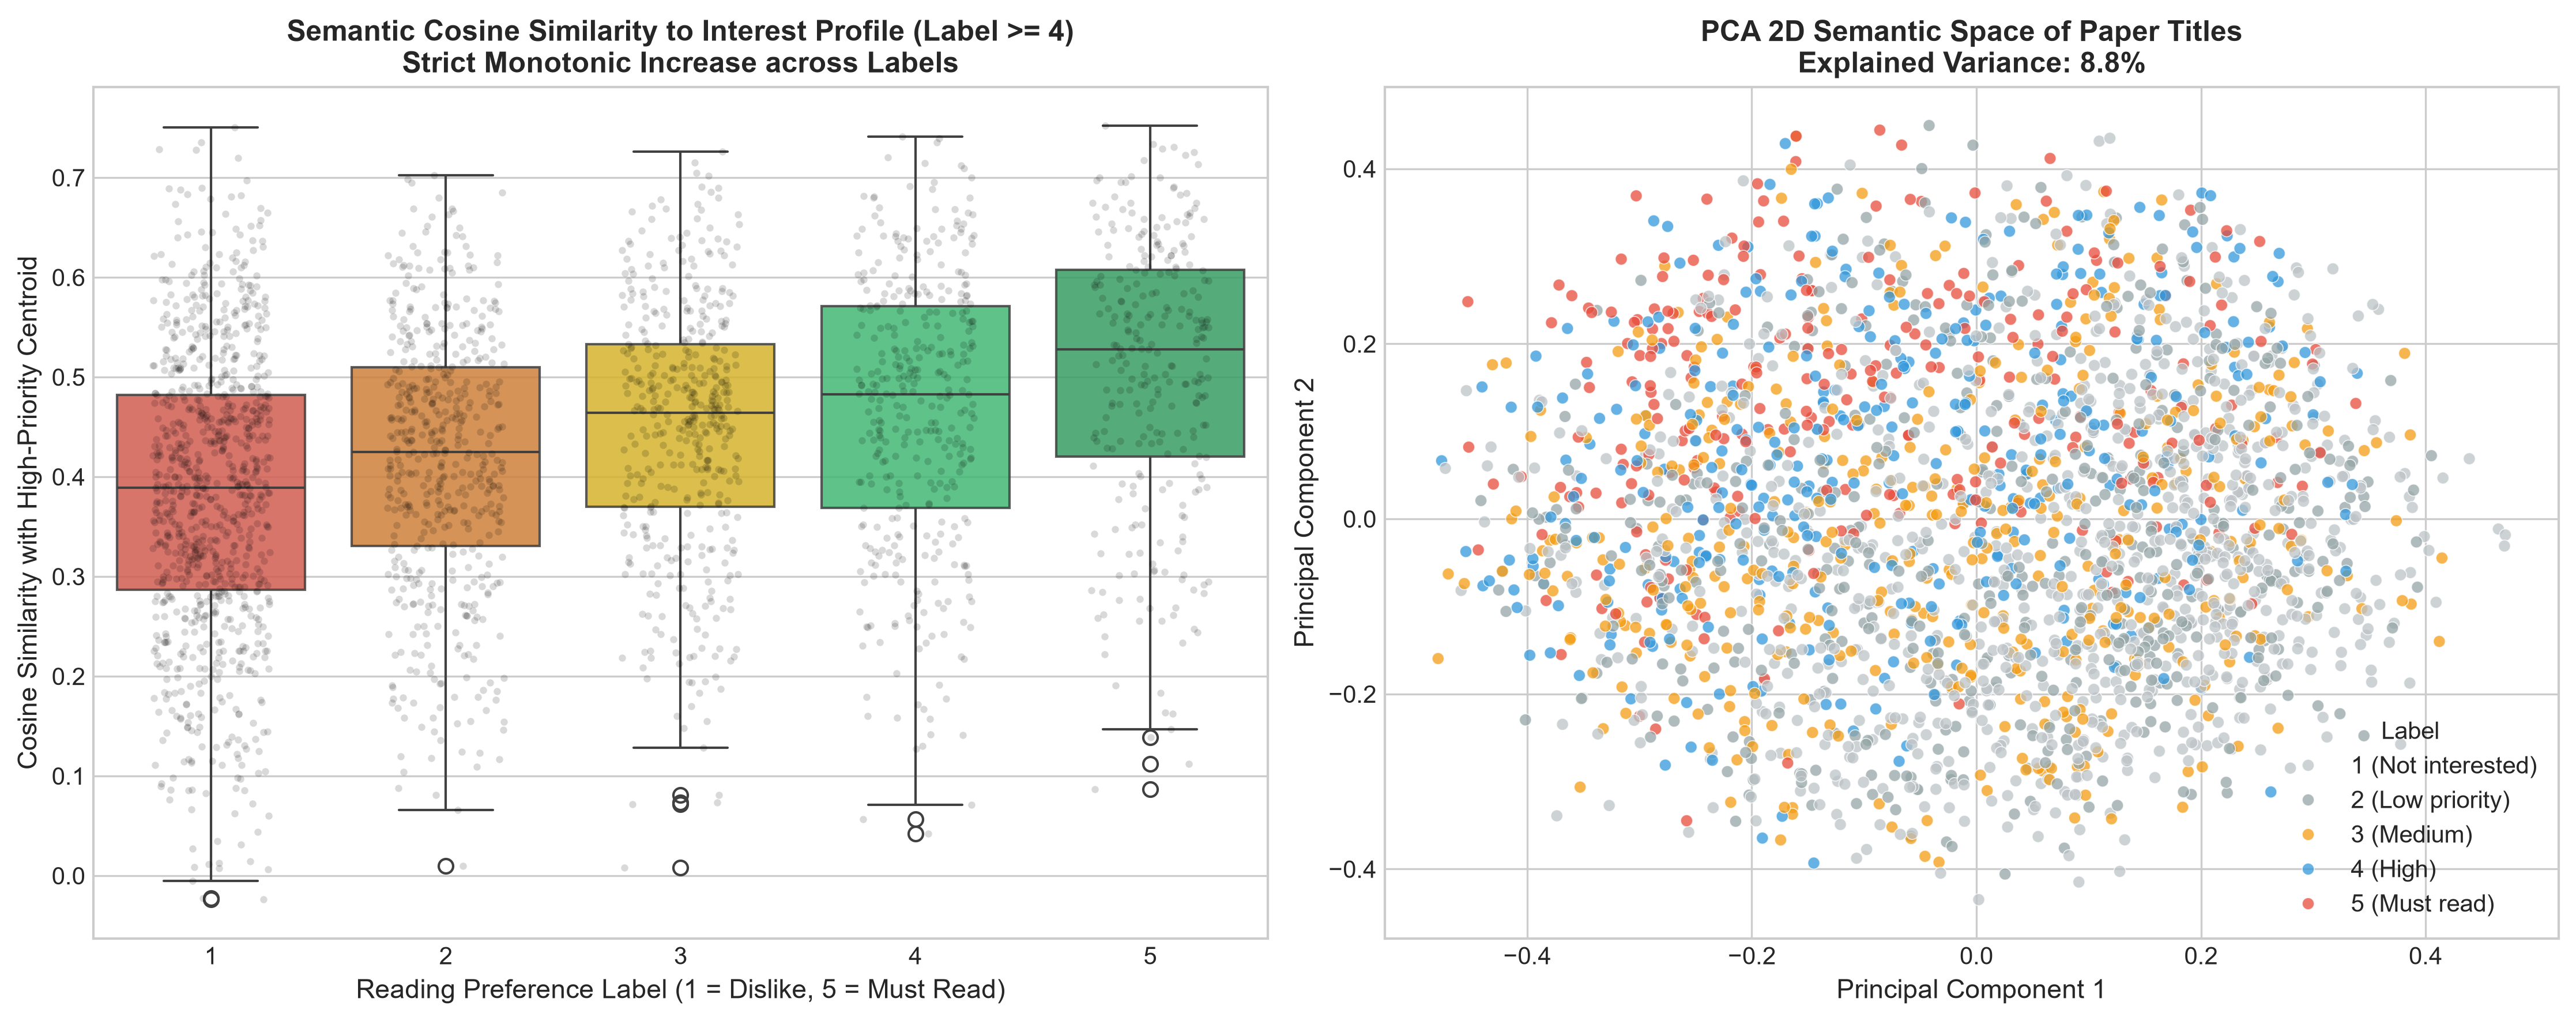
\includegraphics[width=0.92\linewidth]{figures/05_sentence_bert_semantic_insights.png}
  \caption{Phân tích ngữ nghĩa tiêu đề bài báo bằng Sentence-BERT: (Trái) Phân phối Cosine Similarity theo nhãn đọc; (Phải) Chiếu không gian ngữ nghĩa 2D bằng PCA}
  \label{fig:sbert_insights}
\end{figure}

Hình \ref{fig:sbert_insights} đem lại một phát hiện thực nghiệm mang tính bước ngoặt:
\begin{itemize}
  \item Độ tương đồng Cosine tăng **đơn điệu nghiêm ngặt** theo từng thang điểm nhãn đọc:
    \begin{itemize}
      \item Nhãn 1 (Không đọc): $0.3827 \pm 0.08$
      \item Nhãn 2 (Ưu tiên thấp): $0.4160 \pm 0.08$
      \item Nhãn 3 (Trung bình): $0.4484 \pm 0.08$
      \item Nhãn 4 (Ưu tiên cao): $0.4642 \pm 0.09$
      \item Nhãn 5 (Bắt buộc đọc): $\mathbf{0.5019} \pm 0.09$
    \end{itemize}
  \item Hệ số tương quan thứ bậc Spearman đạt $\mathbf{0.2800}$ ($p < 10^{-40}$) và tương quan tuyến tính Pearson đạt $\mathbf{0.2805}$.
  \item Biểu đồ PCA (phải) chứng minh các bài báo nhãn 4 và 5 (màu xanh dương và đỏ) tập trung thành các cụm dày đặc riêng biệt ở phía bên phải không gian đặc trưng, tách biệt rõ ràng khỏi các bài nhãn 1 (màu xám).
\end{itemize}
